\documentclass{standalone}

\usepackage{hyperref}
\usepackage{graphicx}
\usepackage{amsmath}
\usepackage{amssymb}
\usepackage{lmodern}
\usepackage{tikz}
\usetikzlibrary{shapes.geometric,shapes.arrows,decorations.pathmorphing,decorations.markings}
\usetikzlibrary{matrix,chains,scopes,positioning,arrows,fit,spy}
\usepackage{pgfplots}
\pgfplotsset{width=10cm,compat=1.9}
\usepgfplotslibrary{external}

\begin{document}

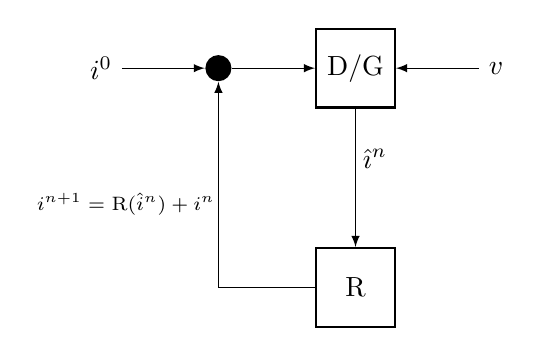
\begin{tikzpicture}[auto, >=latex]
\node (dg) at (0,0) [draw, thick, minimum size=1cm] {$\text{D/G}$};
\node (r) at (dg.south) [draw, thick, minimum width=1cm, minimum height=1cm, below=50pt] {$\text{R}$};
\node (v) at (dg.east) [right=30pt] {$v$};
\node (replace) at (dg.west) [circle, fill=black, minimum size=0.2cm, left=30pt]{};
\node (i0) at (replace.west) [left=30pt]{$i^0$};

\draw [->] (dg) -- (r) node [midway, above=0pt, xshift=7pt] {$\hat{\imath}^n$};
\draw [->] (v) -- (dg) node{};
\draw [->] (i0) -- (replace) node {};
\draw [->, to path={-| (\tikztotarget)}] (r) edge (replace) node [xshift=-83pt, yshift=30pt, font=\scriptsize]{$i^{n+1} = \text{R}(\hat{i}^n) + i^n$};
\draw [->] (replace) -- (dg) node {};
\end{tikzpicture}

\end{document}